\documentclass[Report.tex]{subfiles}

\begin{document}

\chapter{Test and Result}

\section{\textit{LTEWatch} Prototype Board - Power-On}

Before diving in the \textit{LTEWatch} prototype board, modification, power-on and testing, It seems important to specify that the prototypes \textit{PCB} were ordered from \textsc{Euro Circuits} fully assembled. As mentioned on page \pageref{sec:comp_size_select}, many components of the \textit{LTEWatch} prototype board were selected in \textit{BGA} or similar tiny packages in order to design a hardware solution as compact as possible.

\subsection{Prototype Board Objectives}
An important aspect of the project is to assembly and validate a proof of concept prototype board. This prototype board has the following objectives:

\begin{enumerate}
\item \textbf{Concept Validation:}
\begin{itemize}
\item Proof of concept to validate device hardware design
\end{itemize}
\item \textbf{Software Development:} 
\begin{itemize}
\item Functional development board for software experimentation and implementation
\end{itemize}
\item \textbf{Performance Testing:} 
\begin{itemize}
\item Experimental board for feature and performance testing
\end{itemize}
\item \textbf{RF Design Platform:}
\begin{itemize}
\item Development board for designing and testing custom RF antennas
\end{itemize}
\end{enumerate}

\subsection{Prototype Board Modification}
As expected, before powering-on the prototype board, it is necessary to make some corrections and modifications to the receive boards in order to make them fully operational.

\subsubsection{\textit{BAT\_LVL} ADC Input Pin}
Rooting of the \textit{PCB} was done by \textsc{Steve Gallay} of \textit{HEVS}. To simplify rooting he changed the pin assignment of the \textit{nRF9160} and this change was a good idea. The only problem was that it switched the battery level voltage measurement pin which is an analog input to a digital input pin of the \textit{MCU}. To make battery level monitoring available, it is necessary to modify this connection by connecting the \textit{BAT\_LVL} line to an available \textit{AIN} pin of the \textit{nRF9160}. Because there was not a single \textit{AIN} pin available, I decided to sacrifice the \textit{BTN3} button, which is connected to the \textit{AIN3} pin of the MCU.\\

Schematic of the \textit{BAT\_LVL} signal modification is illustrated on figure \ref{fig:adc_mod}:
\begin{figure}[H]
	\centering
	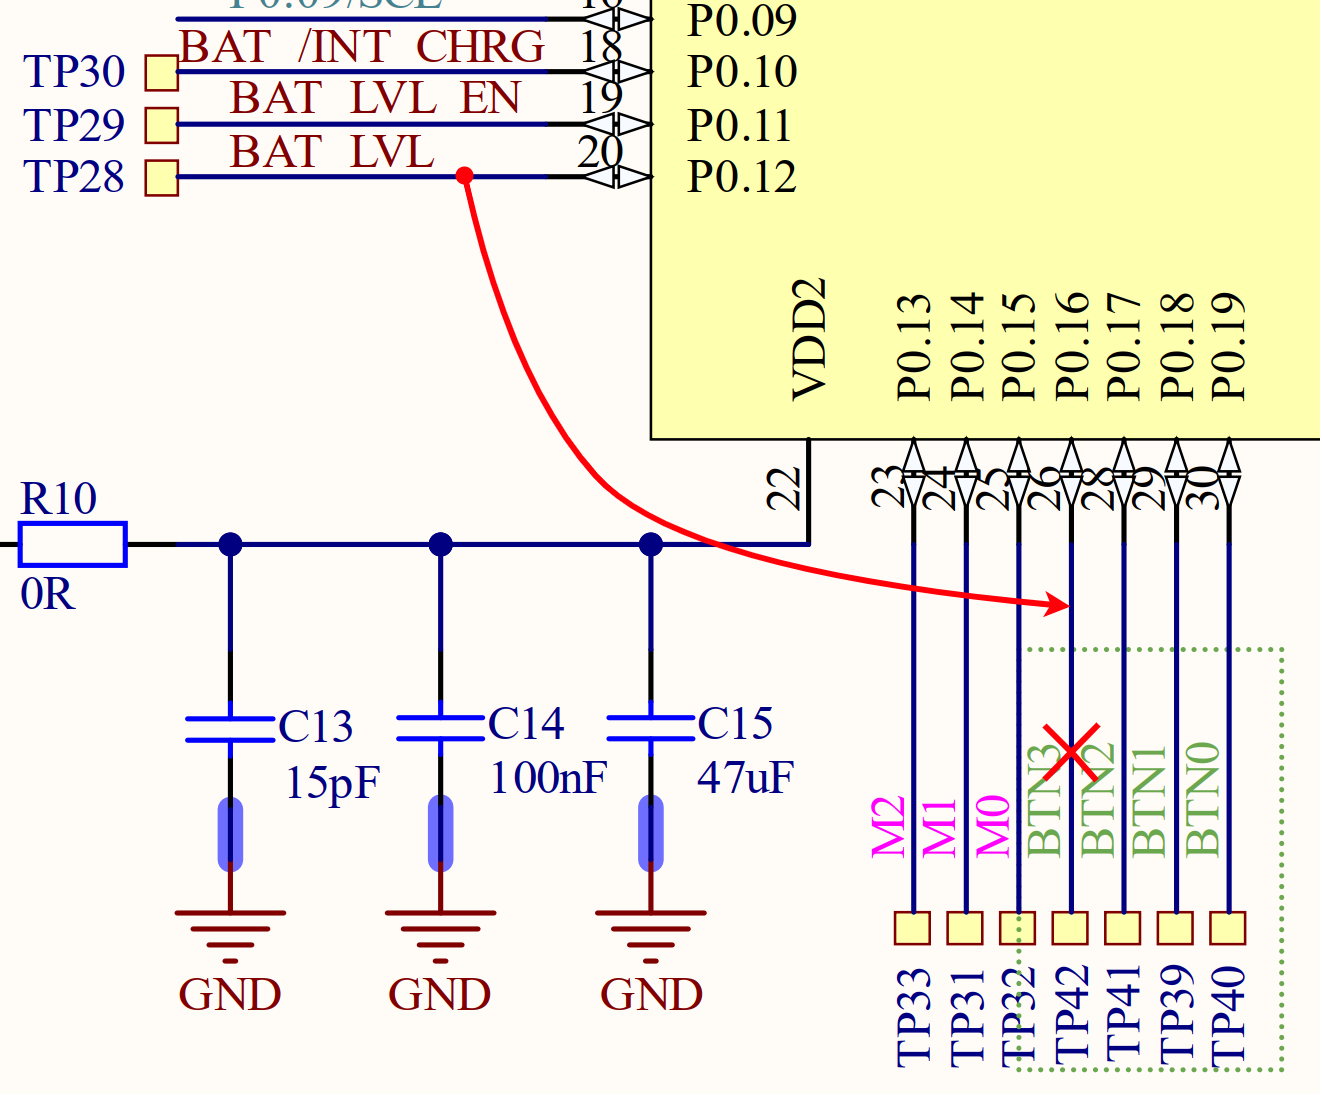
\includegraphics[width=0.8\textwidth]{Include/Figure/modification/adc_mod}
	\caption{\textit{BAT\_LVL} Signal Pin Modification Schematic}
	\label{fig:adc_mod}
\end{figure}

It is also necessary to unplug the power connection to \textit{BTN3} or it will be impossible to measure the battery level. The button debounce capacitor must also be removed to preserve the dynamic characteristic of \textit{BAT\_LVL} signal.\\

The result of the modification (green wire) is illustrated on figure \ref{fig:bord_mod_1}:
\begin{figure}[H]
	\centering
	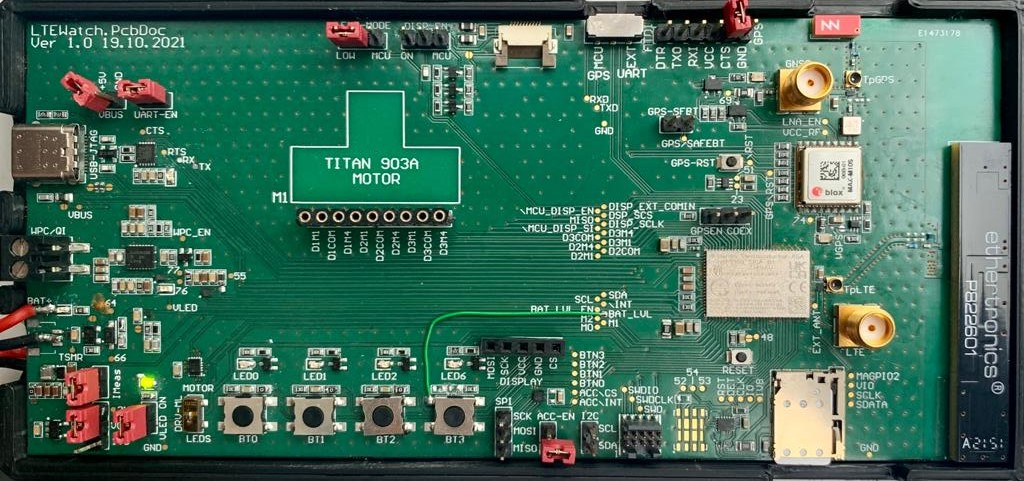
\includegraphics[width=1\textwidth]{Include/Figure/modification/bord_mod_1}
	\caption{Result of the \textit{BAT\_LVL} Signal Pin Modification (Green Wire)}
	\label{fig:bord_mod_1}
\end{figure}

\subsubsection{\textit{Buttons} Interface Modification}
The \textit{buttons} interface of the \textit{user interface} block allows you to choose between several types of button connection with the \textit{MCU}. The chosen configuration requires short-circuiting the series resistors added to the button lines.\\

Schematic of \textit{buttons} interface modification is illustrated on figure \ref{fig:adc_button_mod}:
\begin{figure}[H]
	\centering
	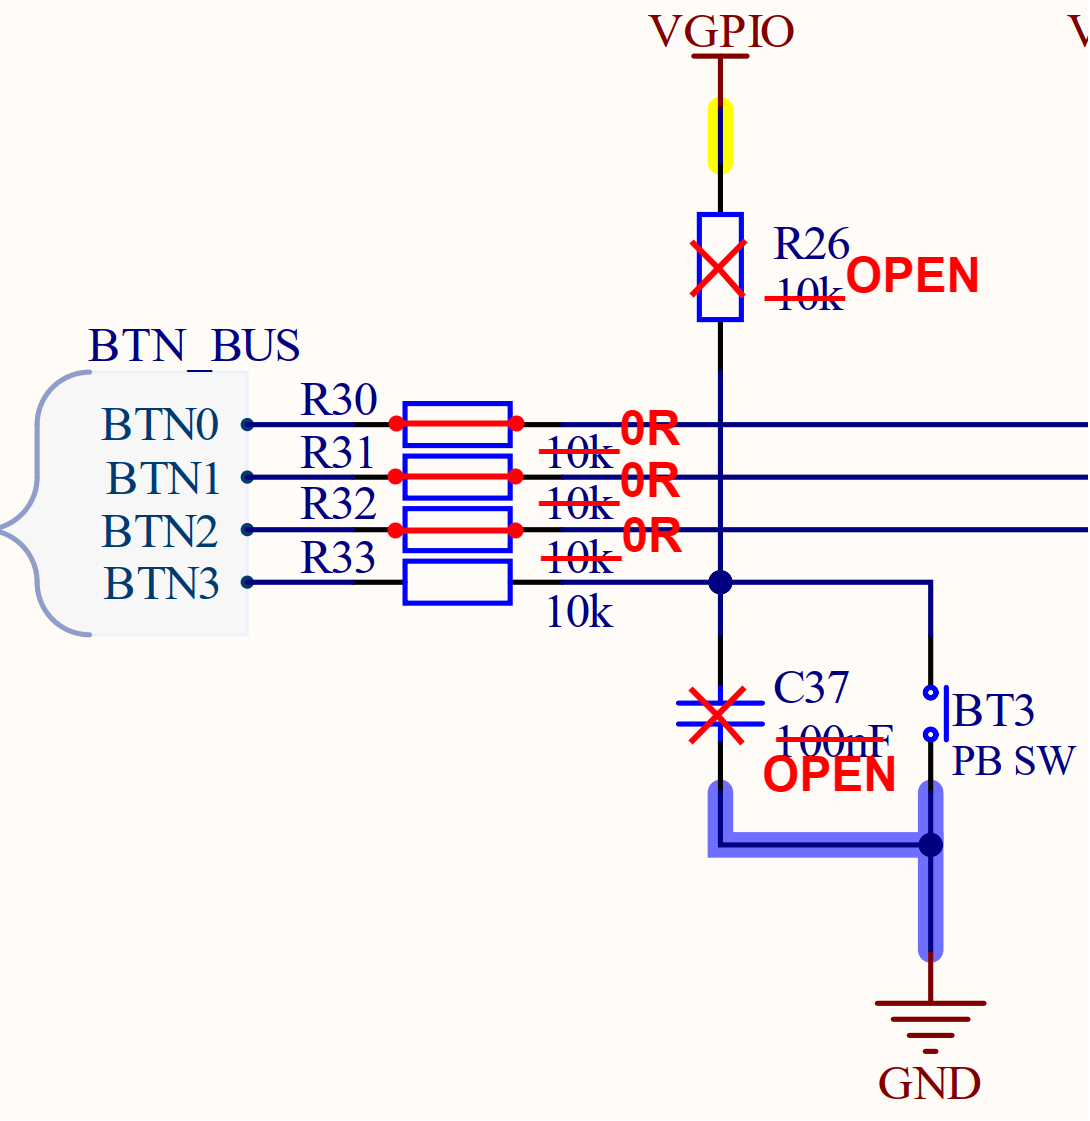
\includegraphics[width=0.6\textwidth]{Include/Figure/modification/adc_button_mod}
	\caption{Schematic of \textit{Buttons} Interface Modification}
	\label{fig:adc_button_mod}
\end{figure}

Figure \ref{fig:adc_button_mod} also illustrates the modifications needed to be processed on \textit{BTN3}.

\subsection{Prototype Board Power-on}
To validate the \textit{LTEWatch} prototype, it is necessary to realize a power-on of the board. To avoid any damage on the board, the power-on process is the following:

\begin{enumerate}
\item \textbf{Battery Charger Unit:}
\begin{enumerate}
\item \textbf{Conditions:}
\begin{enumerate}
\item Jumper \textbf{P5} (\textit{IMEAS}) is disconnected
\item No battery is connected 
\item $R_{65}$ and $R_{73}$ are not mounted (open)
\item Jumper \textbf{P7} (\textit{VGPIO}) is disconnected
\item Jumper \textbf{P6} (\textit{VLED}) is disconnected
\end{enumerate}
\item \textbf{Power-on Process:}
\begin{enumerate}
\item Connect a \SI{5}{\volt} source with current limited to \SI{100}{\milli\ampere} to \textbf{P12} (\textit{VBUS})
\item Measure voltage on \textbf{TP55}
\item Voltage on \textbf{TP55} should be between \ddl{\SI{4.2}{\volt}} and \ddl{\SI{5}{\volt}}
\end{enumerate}
\end{enumerate}
\item \textbf{+3V3 Buck-Boost Converter:}
\begin{enumerate}
\item \textbf{Conditions:}
\begin{enumerate}
\item Jumper \textbf{P5} (\textit{IMEAS}) is connected
\item No battery is connected 
\item $R_{65}$ is mounted
\item $R_{73}$ is mounted
\item Jumper \textbf{P7} (\textit{VGPIO}) is disconnected
\item Jumper \textbf{P6} (\textit{VLED}) is disconnected
\end{enumerate}
\item \textbf{Power-on Process:}
\begin{enumerate}
\item Connect a \SI{5}{\volt} source with current limited to \SI{100}{\milli\ampere} to \textbf{P12} (\textit{VBUS})
\item Measure voltage on the \textbf{+3V3} pin of jumper \textbf{P7} (\textit{VGPIO})
\item Voltage on \textbf{+3V3} pin should be \ddl{\SI{3.3}{\volt}}
\end{enumerate}
\end{enumerate}
\item \textbf{+1V8 LDO Regulator:}
\begin{enumerate}
\item \textbf{Conditions:}
\begin{enumerate}
\item Same as for \textit{+3V3 Buck-Boost Converter}
\end{enumerate}
\item \textbf{Power-on Process:}
\begin{enumerate}
\item Connect a \SI{5}{\volt} source with current limited to \SI{100}{\milli\ampere} to \textbf{P12} (\textit{VBUS})
\item Measure voltage on the \textbf{+1V8} pin of jumper \textbf{P7} (\textit{VGPIO})
\item Voltage on \textbf{+1V8} pin should be \ddl{\SI{1.8}{\volt}}
\end{enumerate}
\end{enumerate}
\item \textbf{USB-C Connector:}
\begin{enumerate}
\item \textbf{Conditions:}
\begin{enumerate}
\item Same as for \textit{+3V3 Buck-Boost Converter}
\end{enumerate}
\item \textbf{Power-on Process:}
\begin{enumerate}
\item Connect a \textbf{USB-C cable} to connector \textbf{J1} (\textit{USB-C}) of the board
\item Measure voltage on the \textbf{+3V3} pin of jumper \textbf{P7} (\textit{VGPIO})
\item Voltage on \textbf{+3V3} pin should be \ddl{\SI{3.3}{\volt}}
\item Measure voltage on the \textbf{+1V8} pin of jumper \textbf{P7} (\textit{VGPIO})
\item Voltage on \textbf{+1V8} pin should be \ddl{\SI{1.8}{\volt}}
\end{enumerate}
\end{enumerate}
\item \textbf{Supply the \textit{nRF9160}}
\begin{enumerate}
\item Bridge \textbf{middle} pin and \textbf{+3V3} pin of jumper \textbf{P7}
\item Bridge \textbf{P5} (\textit{IMEAS})
\item Flash the \textit{nRF9160} using connector \textbf{J2} (\textit{Segger J-Link SWO JTAG}) 
\end{enumerate}
\end{enumerate}

\subsection{\textit{LTEWatch} Board Power-On Result:}

The result of \textit{LTEWatch} board power-on process is described in table \ref{tab:poweron_tab}:

\begin{table}[H]
\centering
\begin{tabularx}{\textwidth}{|X|X|c|c|c|c|}
\hline
\textbf{BLOCK} & \textbf{TP} & \textbf{EXPECTED} & \textbf{MESURED} & \textbf{UNIT} & \textbf{OK/KO} \\\hline
\textit{Battery Charger Unit} & TP55 & $4.20\ldots 5.00$ & $4.36$ & \si{\volt} & \textcolor{mygreen}{OK}\\\hline
\textit{+3V3 Buck-Boost Converter} & \textit{+3V3} of P7 & $3.310$ & $3.$ & \si{\volt} & \textcolor{mygreen}{OK}\\\hline
\textit{+1V8 LDO Regulator} & \textit{+1V8} of P7 & $1.8$ & $1.810$ & \si{\volt} & \textcolor{mygreen}{OK}\\\hline
\textit{USB-C Connector} & \textit{+3V3} of P7 & $3.30$ & $3.312$ & \si{\volt} & \textcolor{mygreen}{OK}\\\hline
\textit{USB-C Connector} & \textit{+1V8} of P7& $1.8$ & $1.807 $ & \si{\volt} & \textcolor{mygreen}{OK}\\\hline
\end{tabularx}
\caption{\textit{LTEWatch} Board Power-On Process Result Table}
\label{tab:poweron_tab}
\end{table}

As shown in table \ref{tab:poweron_tab} the power-on of \textit{LTEWatch} prototype board is a success. The next steps are validation of the specifications of the prototype board.

\pagebreak

\section{\textit{LTEWatch} Prototype - Test \& Validation}
Once the \textit{LTEWatch} prototype board has been successfully powered-on, it is possible to validate the prototype board features that were successfully implemented, based on the prototype specification described on page \ref{sec:specification}.

\begin{table}[H]
\centering
\begin{tabularx}{\textwidth}{|l|X|c|}
\hline
\textbf{BLOCK} & \textbf{SPECIFICATION}  &\textbf{OK/KO} \\\hline
\multirow{3}{*}{Power supply} & Powered by a battery  & \textcolor{mygreen}{OK} \\\cline{2-3}
 & Rechargeable by USB-C and \textit{WPC}  & \textcolor{mygreen}{OK} \\\cline{2-3}
  & Battery life of at least one day  & \textcolor{mygreen}{OK} \\\hline
\multirow{2}{*}{Data Display} & Time is displayed with 3 clock hands & \textcolor{mygreen}{OK} \\\cline{2-3}
  & LCD must be implemented & \textcolor{mygreen}{OK} \\\hline
\multirow{2}{*}{User Interface}  & The user interface must be done with four push-buttons & \textcolor{orange}{OK} \\\cline{2-3}
 & Accelerometer can be added & \textcolor{orange}{OK} \\\hline
Computing Unit & Must use the \textbf{nRF9160} & \textcolor{mygreen}{OK} \\\hline
\multirow{4}{*}{RF Communication} & Must implement a GNSS receiver & \textcolor{mygreen}{OK} \\\cline{2-3}
 & Must implement an LTE-M / NB-IoT transceiver & \textcolor{mygreen}{OK} \\\cline{2-3}
  & Must have on-board antenna for both GNSS and LTE-M & \textcolor{mygreen}{OK} \\\cline{2-3}
   & Must have SMA connectors for GNSS and LTE-M & \textcolor{mygreen}{OK} \\\hline
Mechanical Specification & Build a prototype board & \textcolor{mygreen}{OK} \\\hline
\end{tabularx}
\caption{\textit{LTEWatch} Specifications Validation}
\label{tab:poweron_tab}
\end{table}

As shown on table \ref{tab:poweron_tab}, most specifications are satisfied, the only two that are completely satisfied are:
\begin{enumerate}
\item \textbf{The user interface must be done with four push-buttons:}\\
This specification is not entirely satisfied because one of the buttons have been sacrificed because of a rooting mistakes. The board still implements three fully programmable and functional buttons, \textit{BT0, BT1} and \textit{BT2}.

\item \textbf{Accelerometer can be added:}
due to the limited time available, the accelerometer could not be implemented during the project. On the other hand, the accelerometer is integrated on the board and the \textit{SPI} communication is already implemented for the display. The only remaining tasks are only software development tasks, which are importing a suitable driver for the accelerometer and to add it to the small watch application.
\end{enumerate}

\pagebreak

\subsection{Validation of the Display}
The display is fully implemented and functional. To validate its implementation, \textit{LTEWatch} application start-up process is demonstrated bellow:

\begin{enumerate}
\item \textbf{Connect the battery to the board}
\item \textbf{\textit{LTEWatch} is in \textit{Set Motor Position} mode:}
\begin{figure}[H]
	\centering
\begin{subfigure}{.3\textwidth}
\centering
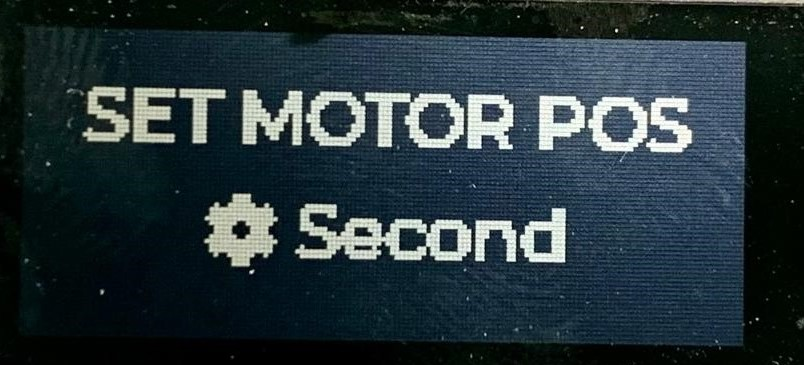
\includegraphics[width=1\textwidth]{Include/Figure/modification/display_1}
\caption{Set Second}
\end{subfigure}	
\begin{subfigure}{.3\textwidth}
\centering
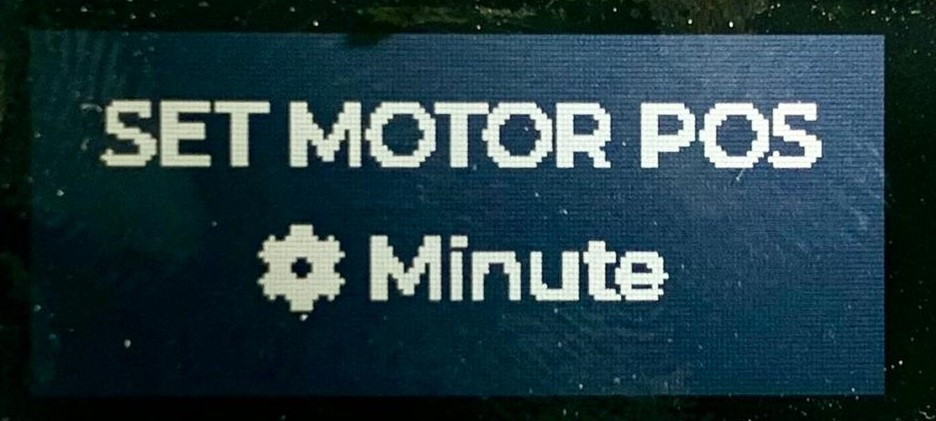
\includegraphics[width=1\textwidth]{Include/Figure/modification/display_2}
\caption{Set Minute}
\end{subfigure}	
\begin{subfigure}{.3\textwidth}
\centering
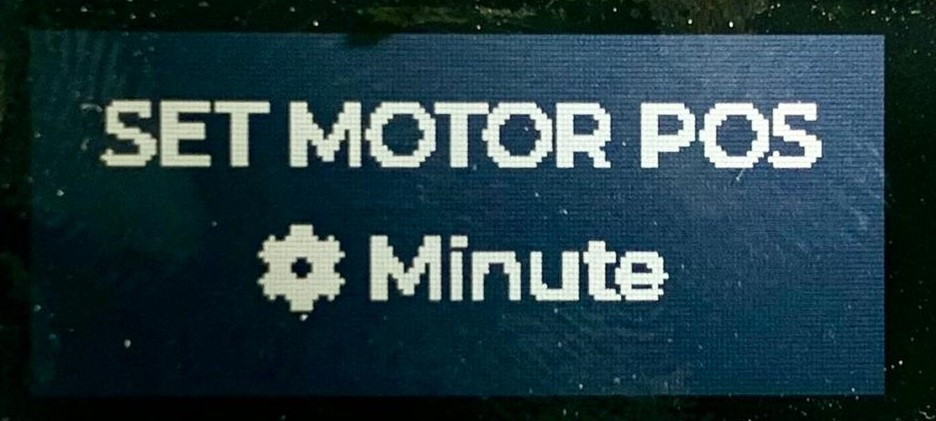
\includegraphics[width=1\textwidth]{Include/Figure/modification/display_2}
\caption{Set Hour}
\end{subfigure}	
	\caption{Display Test - Set Motor Position}
	\label{fig:display_1}
\end{figure}
\begin{itemize}
\item Click \textit{BT1}: Move selected clock hands 1 step clockwise
\item Click \textit{BT0}: Move selected clock hands 1 step counterclockwise
\item Long Press \textit{BT1}: Continuously move selected clock hands clockwise
\item Long Press \textit{BT0}: Continuously move selected clock hands counterclockwise
\item Double Click \textit{BT1}: Change selected clock hand forward
\item Double Click \textit{BT0}: Change selected clock hand backward
\item Triple Click \textit{BT1}: Save and exit to next mode
\item Triple Click \textit{BT0}: Save and exit to previous mode
\end{itemize}
\item \textbf{\textit{LTEWatch} is in \textit{Set \textit{GNSS} Antenna} mode:}
\begin{figure}[H]
	\centering
\begin{subfigure}{.3\textwidth}
\centering
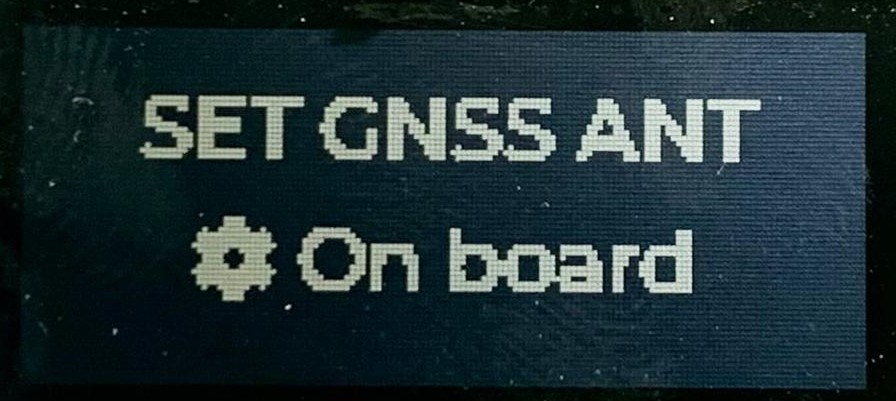
\includegraphics[width=1\textwidth]{Include/Figure/modification/display_4}
\caption{On-board Antenna}
\end{subfigure}	
\begin{subfigure}{.3\textwidth}
\centering
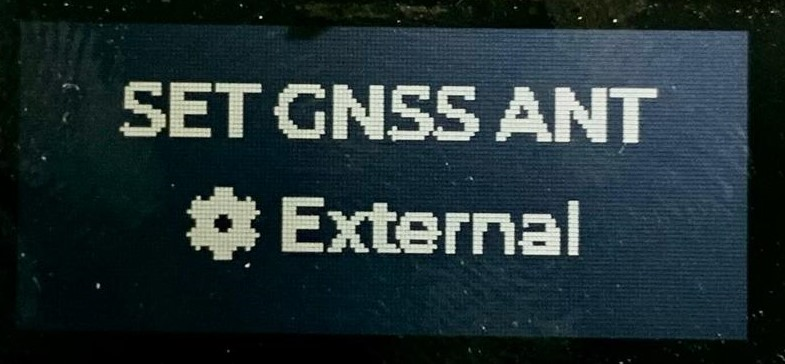
\includegraphics[width=1\textwidth]{Include/Figure/modification/display_5}
\caption{External Antenna}
\end{subfigure}	
	\caption{Display Test - Set \textit{GNSS} Antenna Mode}
	\label{fig:display_1}
\end{figure}

\begin{itemize}
\item Click \textit{BT1}: Select next antenna option
\item Click \textit{BT0}: Select previous antenna option
\item Triple Click \textit{BT1}: Save and exit to next mode
\item Triple Click \textit{BT0}: Save and exit to previous mode
\end{itemize}
\pagebreak
\item \textbf{\textit{LTEWatch} Application is starting up:}
\begin{figure}[H]
	\centering
\begin{subfigure}{.3\textwidth}
\centering
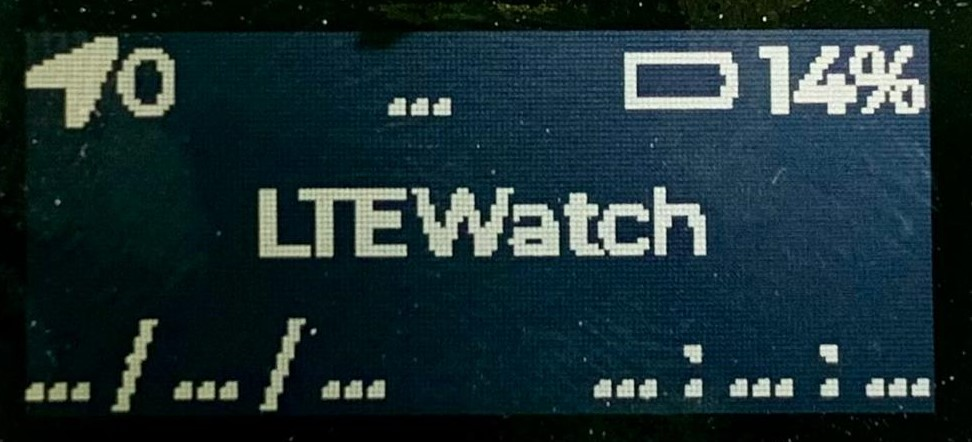
\includegraphics[width=1\textwidth]{Include/Figure/modification/display_6}
\caption{App. Start}
\end{subfigure}	
\begin{subfigure}{.3\textwidth}
\centering
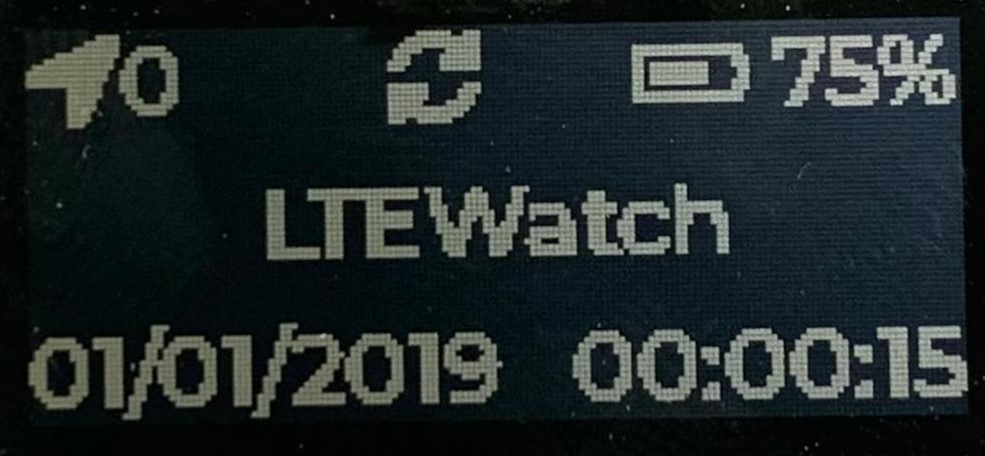
\includegraphics[width=1\textwidth]{Include/Figure/modification/display_7}
\caption{\textit{MQTT} Connecting}
\end{subfigure}	
\begin{subfigure}{.3\textwidth}
\centering
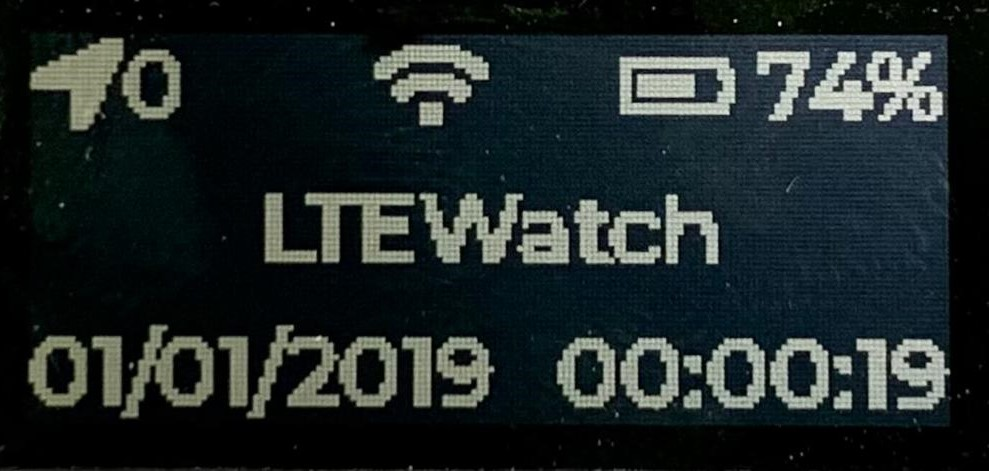
\includegraphics[width=1\textwidth]{Include/Figure/modification/display_8}
\caption{\textit{MQTT} Connected}
\end{subfigure}	
	\caption{Display Test - \textit{LTEWatch} Application Start-Up}
	\label{fig:display_1}
\end{figure}

\item \textbf{\textit{LTEWatch} is in \textit{Normal} mode:}\\
During this mode, the \textit{GNSS} position update and the refresh rate of sending \textit{MQTT} data is determined by the current speed of the device. If the movement speed of the device increases, the refresh rate also increases and if the movement speed of the device decreases, the refresh rate also decreases.
\begin{figure}[H]
	\centering
\begin{subfigure}{.3\textwidth}
\centering
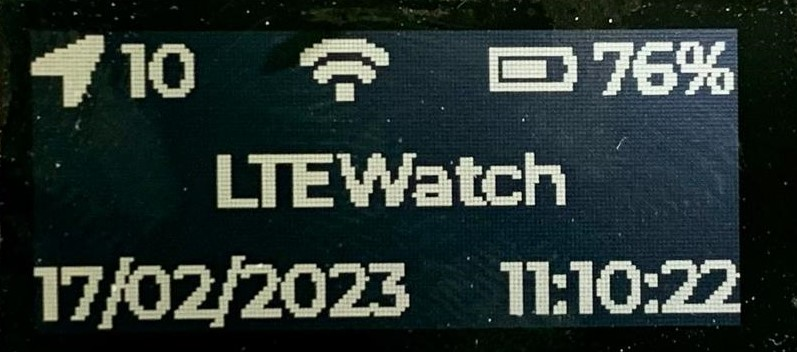
\includegraphics[width=1\textwidth]{Include/Figure/modification/display_9}
\caption{\textit{GNSS} Connected}
\end{subfigure}	
\begin{subfigure}{.3\textwidth}
\centering
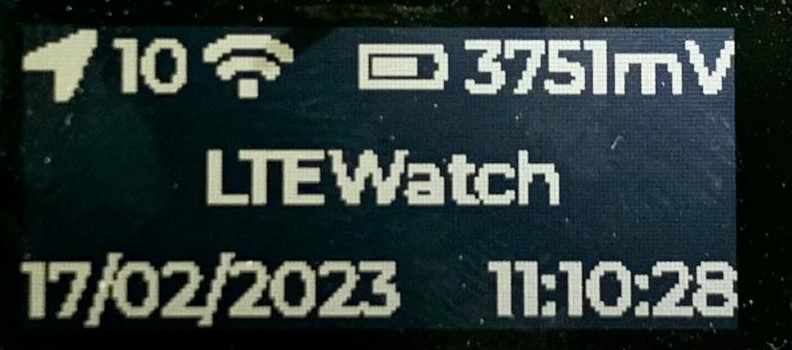
\includegraphics[width=1\textwidth]{Include/Figure/modification/display_10}
\caption{Bat Level In \si{\milli\volt}}
\end{subfigure}	
	\caption{Display Test - Normal Mode}
	\label{fig:display_1}
\end{figure}
\begin{itemize}
\item Click \textit{BT0}: Update time and date value with \textit{GNSS} receiver's data
\item Double Click \textit{BT2}: Change battery level unit (\si{\milli\volt}/\si{\percent})
\item Triple Click \textit{BT2}: Reset battery charger configuration
\item Long Press \textit{BT0}: Change active mode (\textit{Normal/Tracking})
\end{itemize}
\item \textbf{\textit{LTEWatch} is in \textit{Tracking} mode:}
\begin{figure}[H]
	\centering
	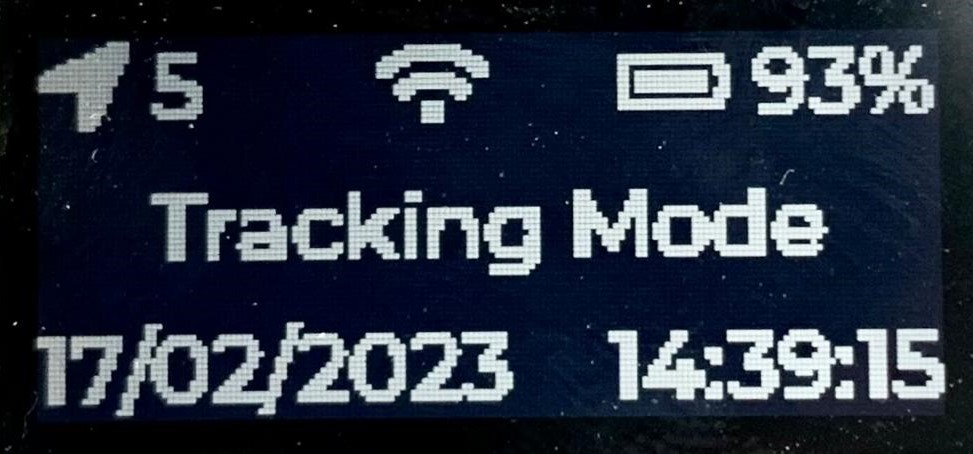
\includegraphics[width=0.3\textwidth]{Include/Figure/modification/display_11}
	\caption{Display Test - Tracking Mode}
	\label{fig:tracking_exemple_1}
\end{figure}
\end{enumerate}
During this mode, the \textit{GNSS} position is updated every second. The \textit{MQTT} data are sent every second as well. 

\pagebreak

\subsection{Validation of \textit{GNSS} and \textit{LTE-M/NB-IoT}}

In order to validate the \textit{GNSS} position, \textit{LTE-M/NB-IoT} and \textit{MQTT} communication, a \textit{Thingsboard} dashboard was created. To do so, \textsc{Patrice Rudaz} help me to log my device on one of \textit{HEVS} servers: \url{https://tb.ecs.hevs.ch/}. Once done, a graphical user interface was created. This dashboard is public and is accessible with this link: \url{https://tb.ecs.hevs.ch/dashboard/4d6aa6b0-9701-11ed-8466-731d9ee1dd28?publicId=4bb1eaf0-ab74-11ec-aeec-99b485820668}.\\

The dashboard display the following information:
\begin{itemize}
\item \textit{GNSS} position tracking on \textit{OpenStreetMap}
\item Number of satellites connected to the \textit{GNSS} receiver of the device (\textit{SVS})
\item Speed of the device
\item Battery level in \si{\percent}
\item Last published altitude of the device
\item \textit{GNSS} Altitude Tracking
\item Battery level in \si{\milli\volt}
\item Graph of published altitude values
\item Graph of published speed values
\item Graph of published \textit{SVS} values
\item Graph of published battery level values\\
\end{itemize}

The created \textit{Thingsboard} dashboard is illustrated in figure \ref{fig:ltewatch_panel}:
\begin{figure}[H]
	\centering
	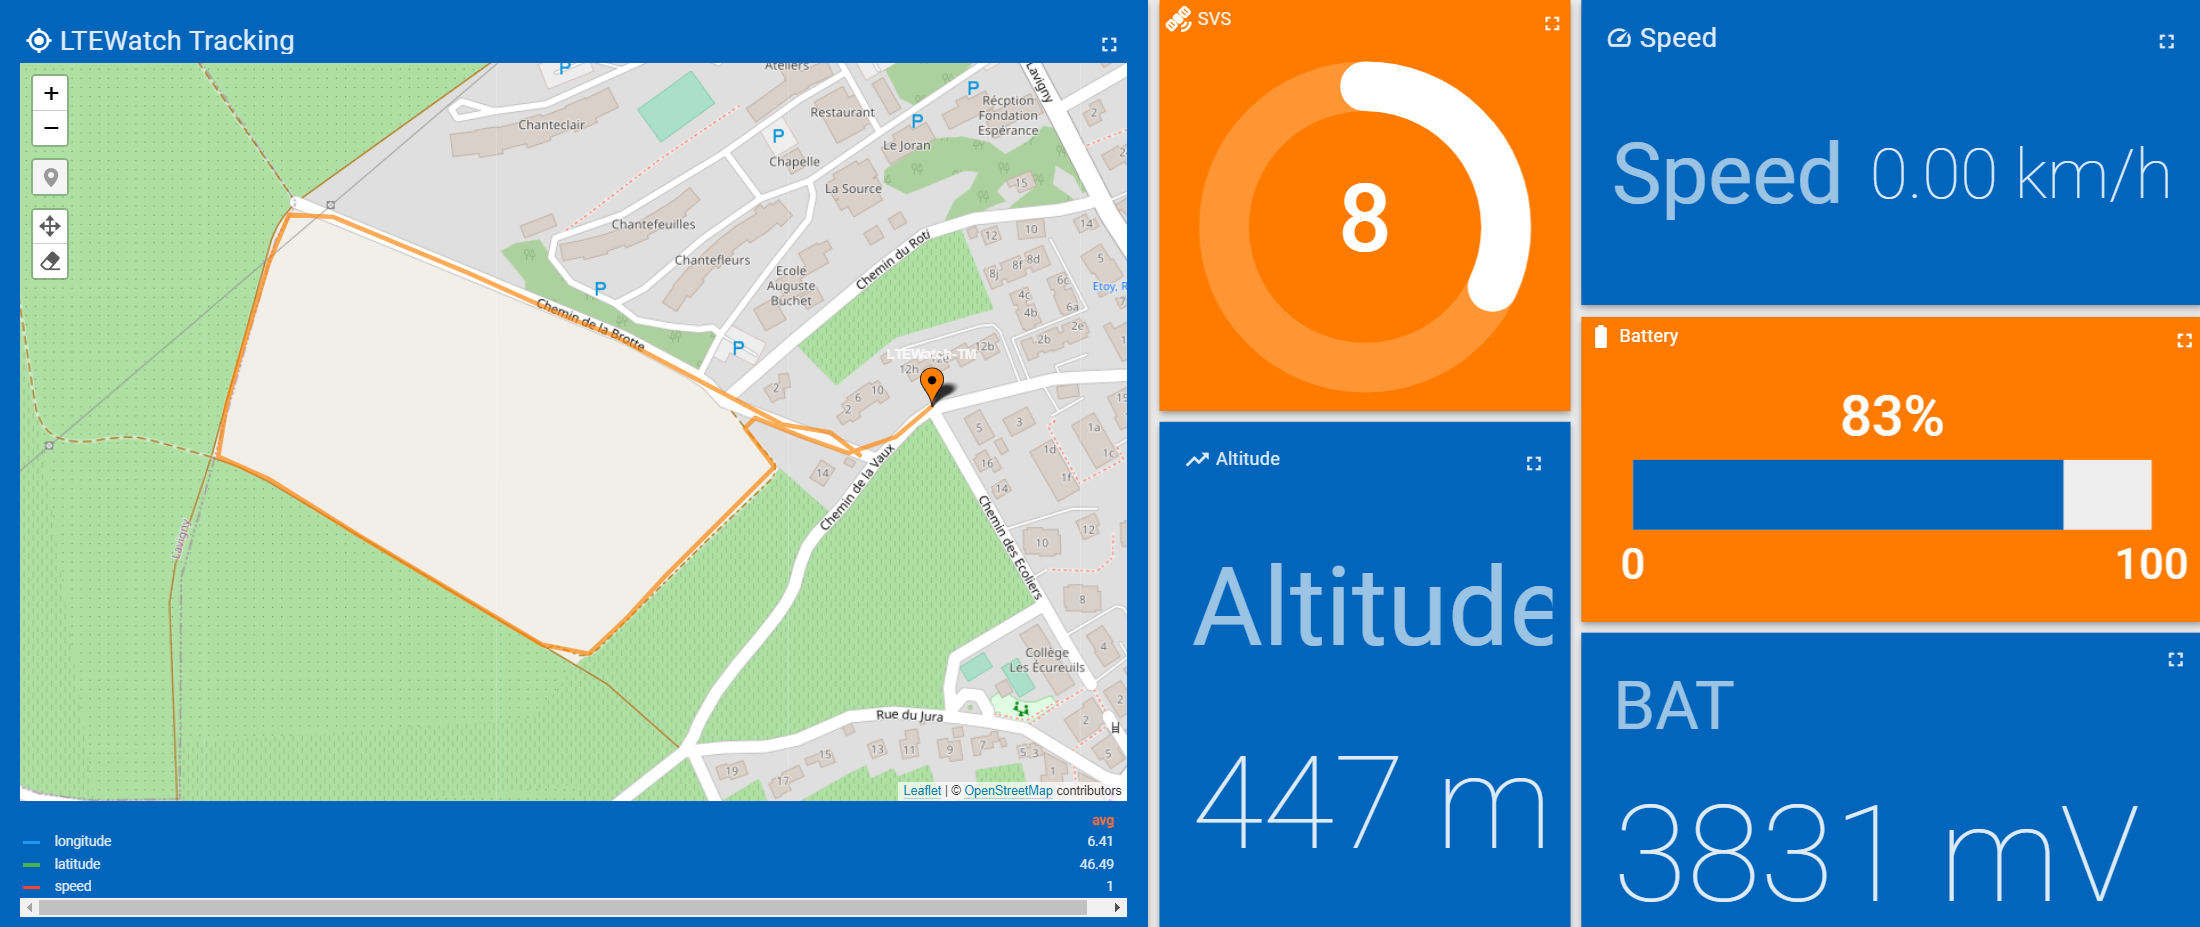
\includegraphics[width=1\textwidth]{Include/Figure/result/ltewatch_panel.png}
	\caption{\textit{LTEWatch} - Dashboard (Thingsboard)}
	\label{fig:ltewatch_panel}
\end{figure}

With the created dashboard illustrated in figure \ref{fig:ltewatch_panel}, it is possible to validate the \textit{GNSS} receiver and the \textit{LTE-M/NB-IoT} modem implementation by testing multiple tracking scenarios.\\

Figures \ref{fig:gnss_accuracy_1} to \ref{fig:gnss_accuracy_2} illustrates the test of the \textit{LTEWatch} prototype board \textit{GNSS} accuracy. This test uses the \textit{LTEWatch} in tracking mode and the on-board \textit{GNSS} antenna and on-board \textit{LTE-M/NB-IoT} antenna:

\begin{figure}[H]
	\centering
	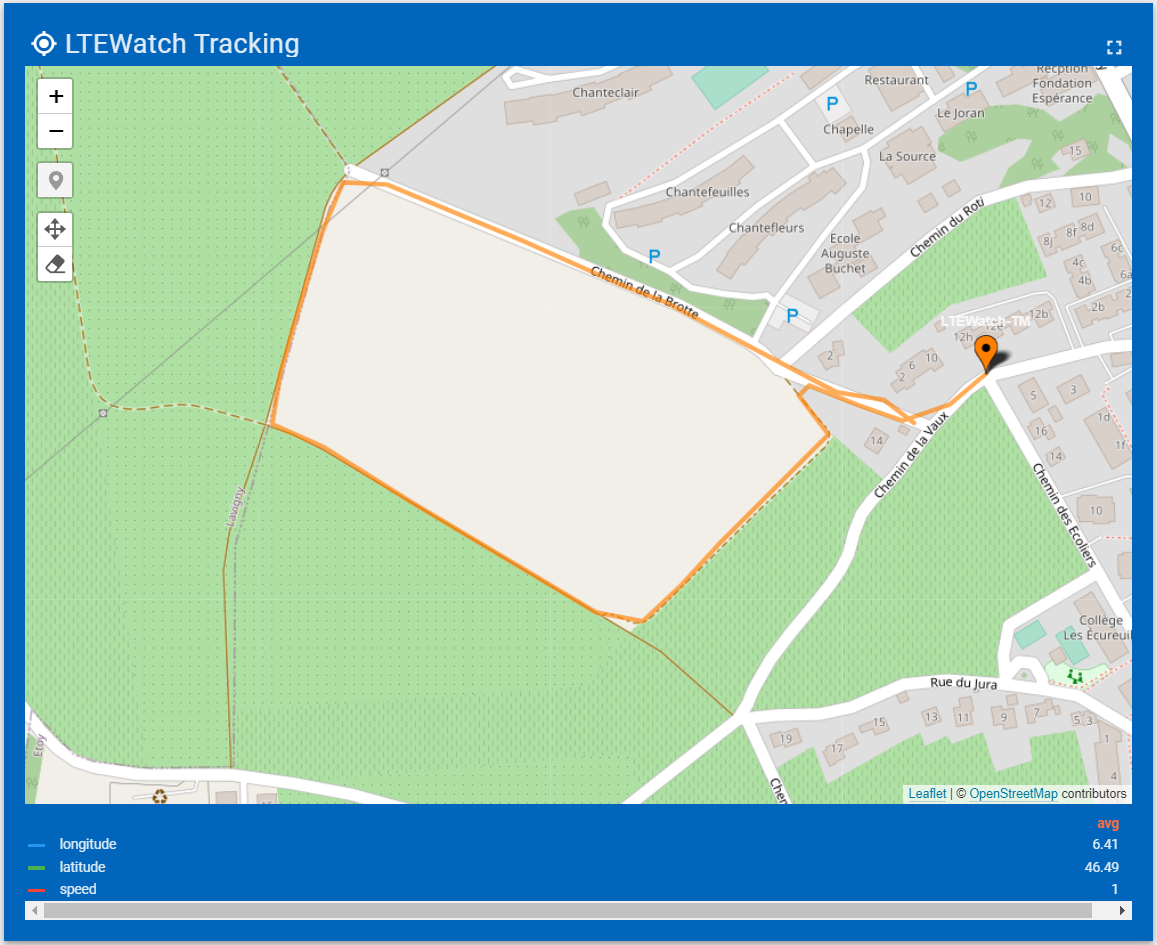
\includegraphics[width=0.8\textwidth]{Include/Figure/result/ltewatch_result_2.png}
	\caption{\textit{LTEWatch} - GNSS Tracking Accuracy}
	\label{fig:gnss_accuracy_1}
\end{figure}

As figure \ref{fig:gnss_accuracy_1} shows, the \textit{GNSS} tracking accuracy is very good, even with the tiny \textit{GNSS} on-board antenna. The tracking line (in orange) follows roads and paths very well. This result is very satisfying and validates the tracking mode of the \textit{LTEWatch} prototype board. The following figure \ref{fig:gnss_accuracy_2} illustrates the altitude tracking that was published during the previous route.

\begin{figure}[H]
	\centering
	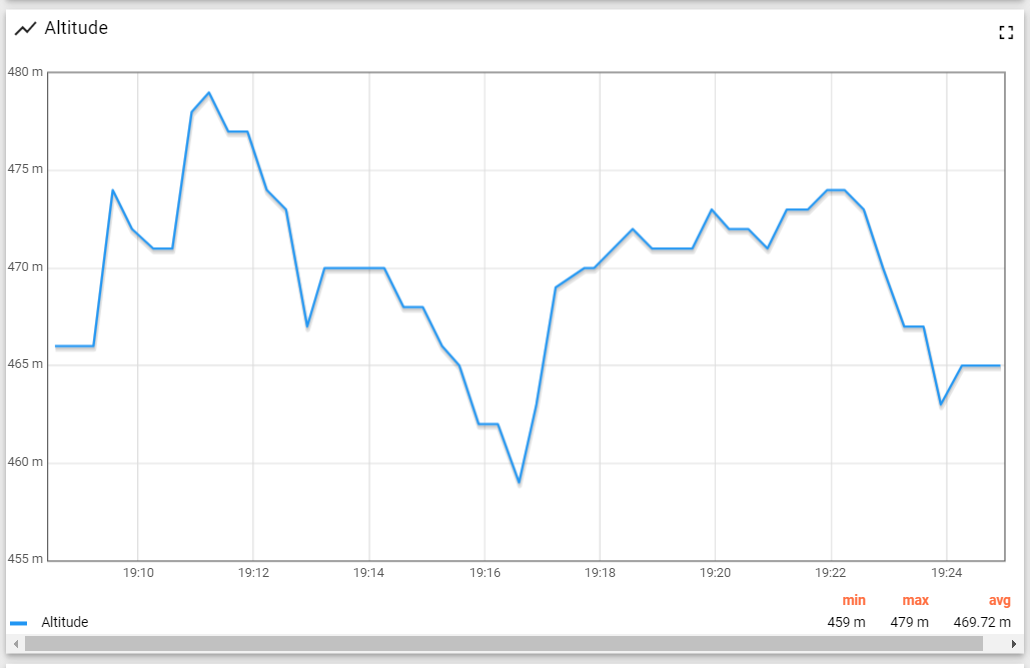
\includegraphics[width=0.7\textwidth]{Include/Figure/result/ltewatch_result_1.png}
	\caption{\textit{LTEWatch} Tracking Test - Altitude Accuracy}
	\label{fig:gnss_accuracy_2}
\end{figure}

Once the tracking mode of the \textit{LTEWatch} prototype board has been validated, it is interesting to try a much more complicated scenario by testing \textit{GNSS} tracking over a long distance journey. The figure \ref{fig:tracking_exemple_1} illustrates the tracking \textit{GNSS} of the trajectory in train from my home to the \textit{HEVS}.

\begin{figure}[H]
	\centering
\begin{subfigure}{.45\textwidth}
\centering
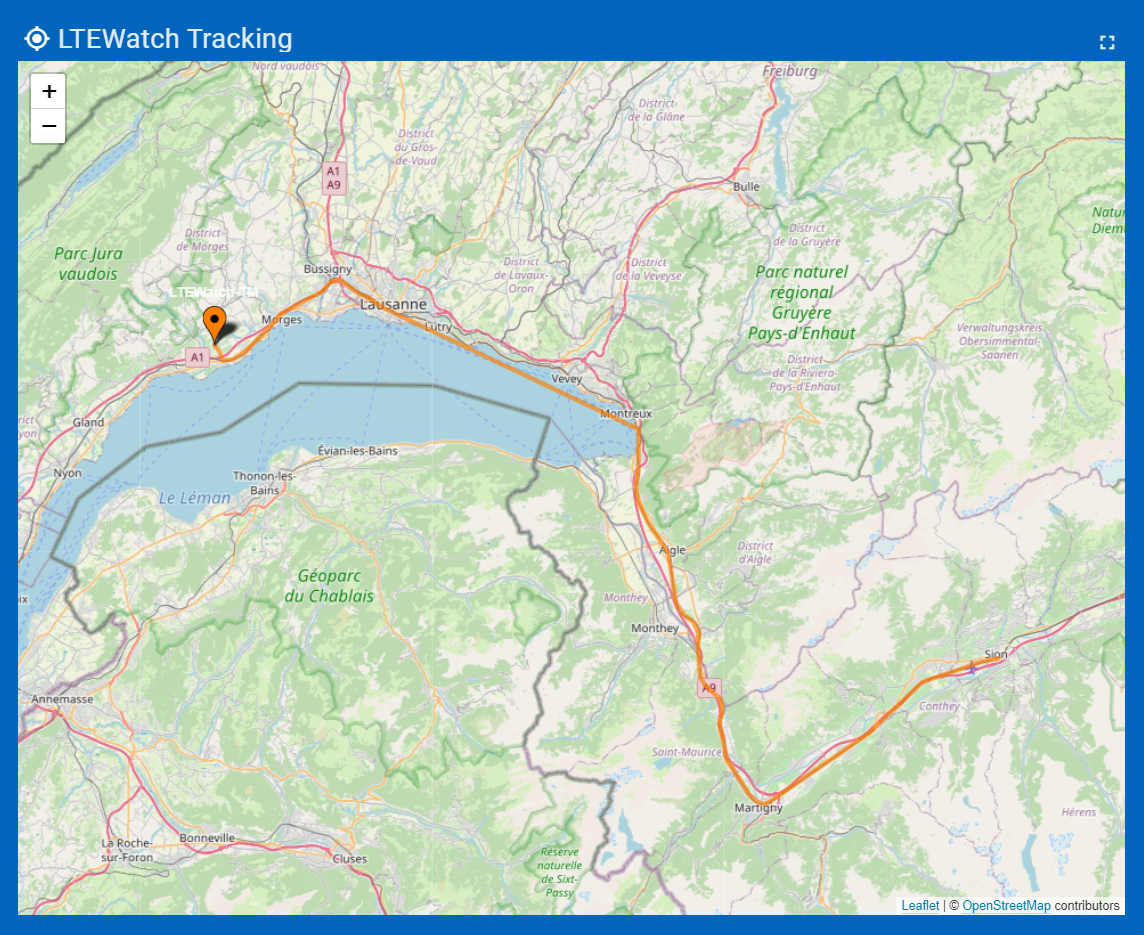
\includegraphics[width=1\textwidth]{Include/Figure/result/tracking_exemple_1.png}
\caption{\textit{GNSS} Position Tracking}
\end{subfigure}	
\begin{subfigure}{.45\textwidth}
\centering
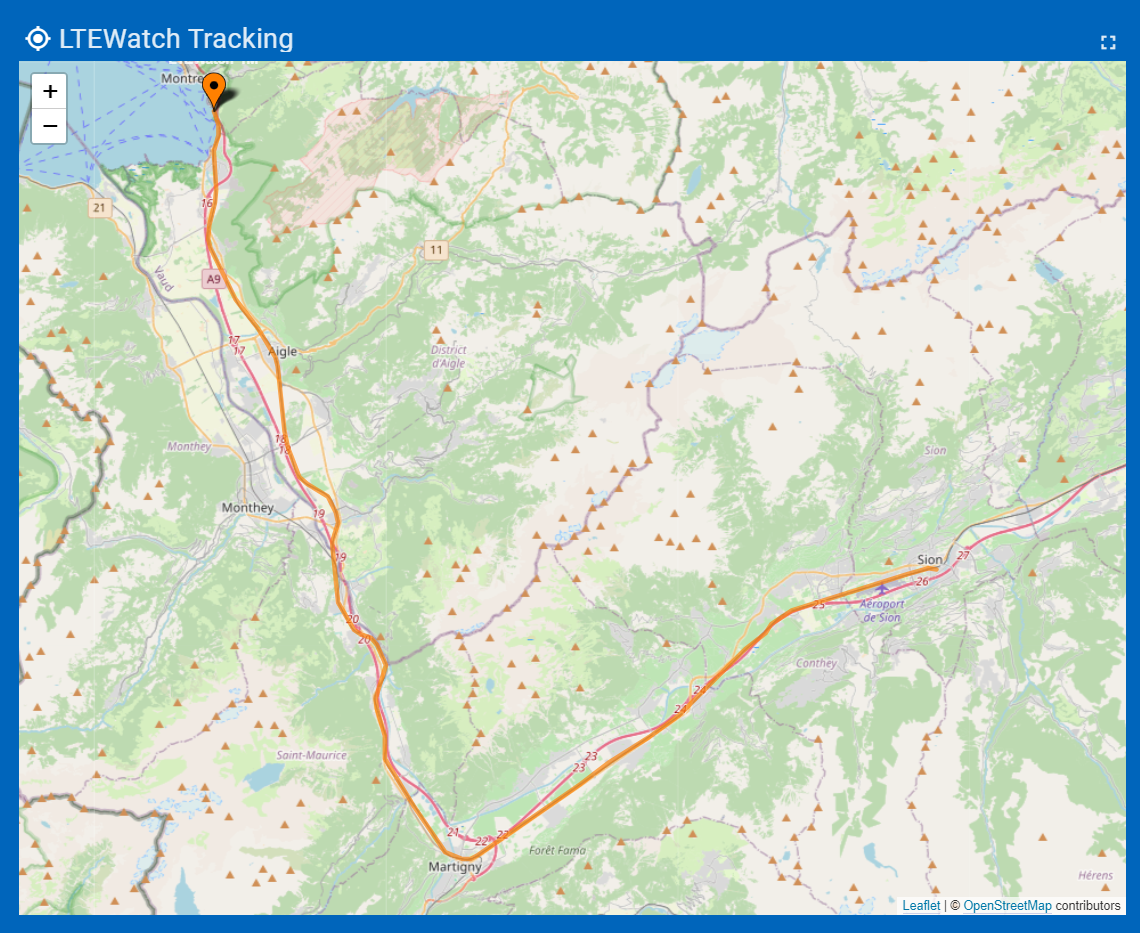
\includegraphics[width=1\textwidth]{Include/Figure/result/tracking_exemple_4.png}
\caption{\textit{GNSS} Position Tracking}
\end{subfigure}	
\begin{subfigure}{.45\textwidth}
\centering
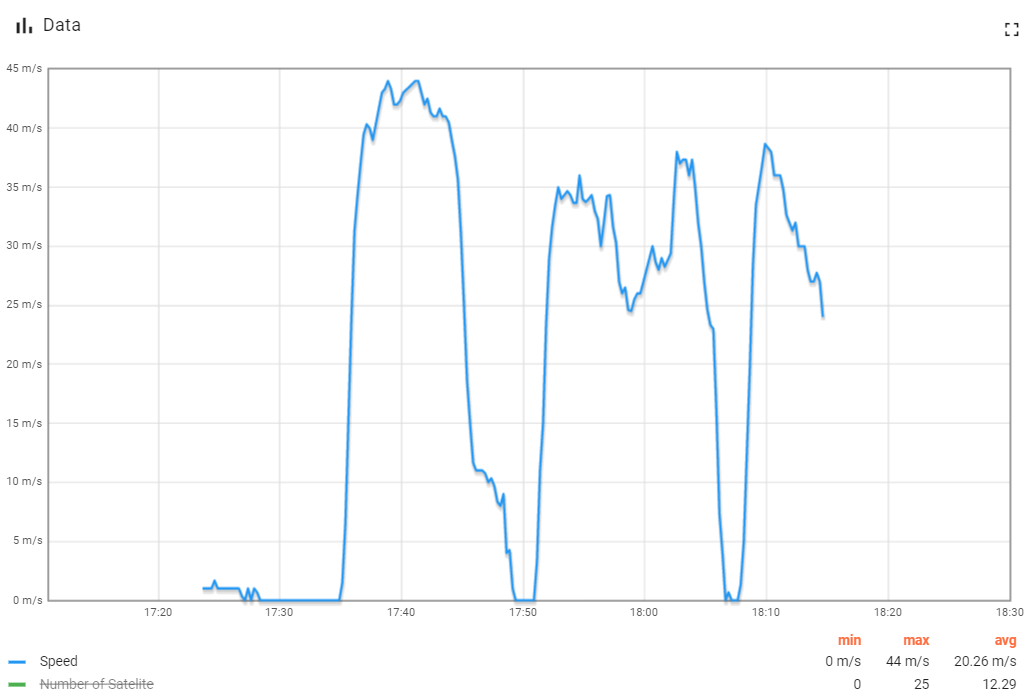
\includegraphics[width=1\textwidth]{Include/Figure/result/tracking_exemple_4_speed.png}
\caption{\textit{GNSS} Speed Tracking}
\end{subfigure}	
\begin{subfigure}{.45\textwidth}
\centering
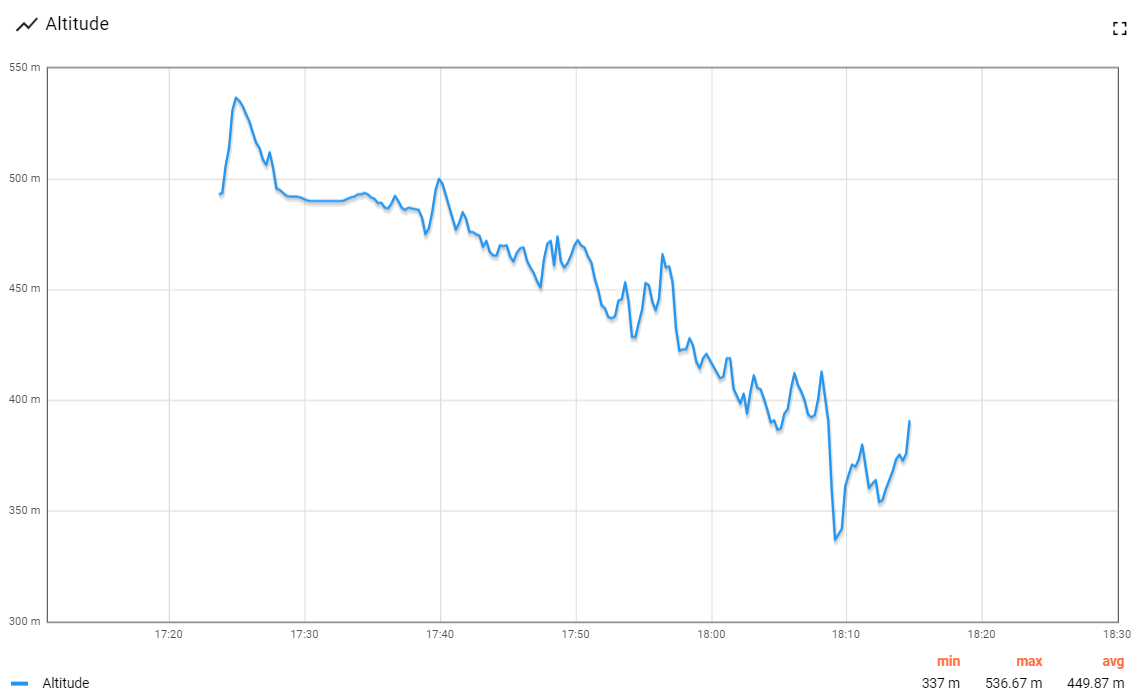
\includegraphics[width=1\textwidth]{Include/Figure/result/tracking_exemple_4_altitude.png}
\caption{\textit{GNSS} Altitude Tracking}
\end{subfigure}	
	\caption{\textit{GNSS} \& \textit{LTE-M/NB-IoT} Validation - Long Distance Tracking}
	\label{fig:tracking_exemple_1}
\end{figure}


\begin{figure}[H]
	\centering
	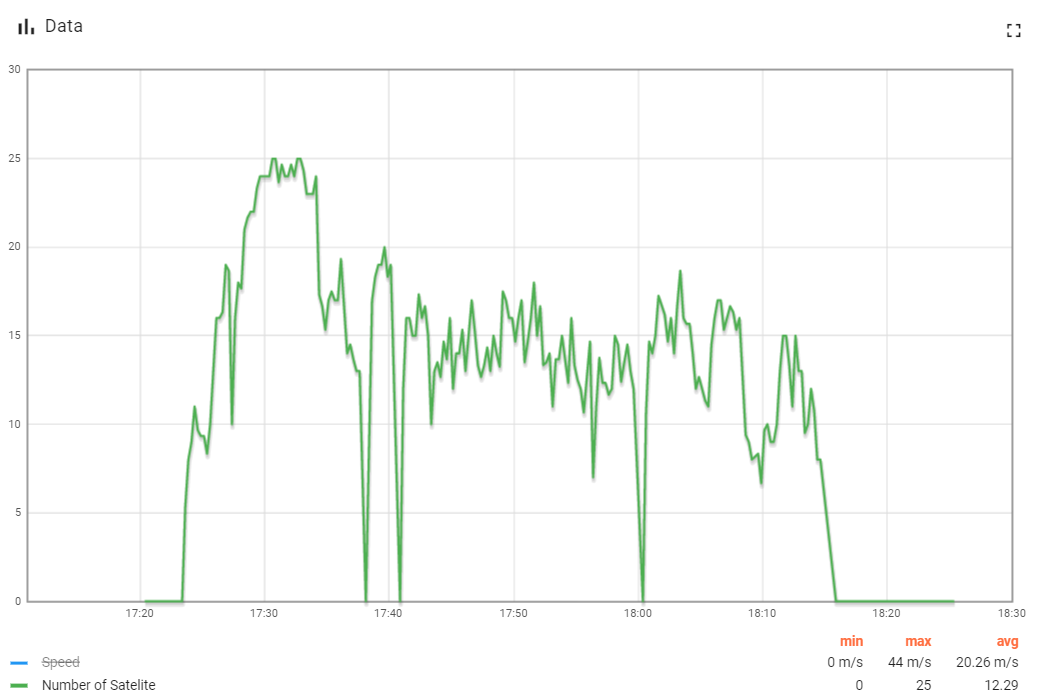
\includegraphics[width=0.7\textwidth]{Include/Figure/result/tracking_exemple_4_svs.png}
	\caption{\textit{GNSS} \& \textit{LTE-M/NB-IoT} Validation - Number of Satellite (\textit{SVS})}
	\label{fig:tracking_exemple_4_svs}
\end{figure}


\end{document}